All tested numerical methods successfully converged to a solution, though their effectiveness and required computational effort varied significantly. 
The FIR filter proved highly effective at noise reduction, successfully handling signals where additive Gaussian noise had a standard deviation as high as 90. 
The subsequent spike detection algorithm demonstrated a precision of 0.75, and recall of 0.6. Overall the $F_1$ score of the algorithm is 0.67.

\subsection{Numerical Methods Performance}
\label{subsec:numerical-methods-results}

    Each numerical integration method required a minimum step size, defined as a ratio of steps to the total simulation time frame, to produce a stable solution. 
    As shown in Table~\ref{tab:min_steps}, the fourth-order Runge-Kutta (RK4) method was the most efficient, converging with the smallest step count.

    \begin{center}
        \captionof{table}{Minimum convergence step ratios}
        \label{tab:min_steps}
        \begin{tabular}{@{}ccc@{}}
        \toprule
        Method & Time (ms) & Steps/ms \\
        \midrule
        Euler & 100 & 17 \\
        Improved Euler & 100 & 19 \\
        RK4 & 100 & 14 \\
        \bottomrule
        \end{tabular}  
    \end{center}

    Beyond efficiency, the accuracy at these minimum convergence thresholds varied drastically. 
    The RK4 method produced a smooth, physically plausible solution curve. 
    In contrast, the Forward Euler method, operating at its minimum step ratio, exhibited significant instability and error accumulation due to the large time step, as visualized in Figure~\ref{fig:euler-min-convergence}.

    \end{multicols}

    \begin{figure}[ht]
        \centering
        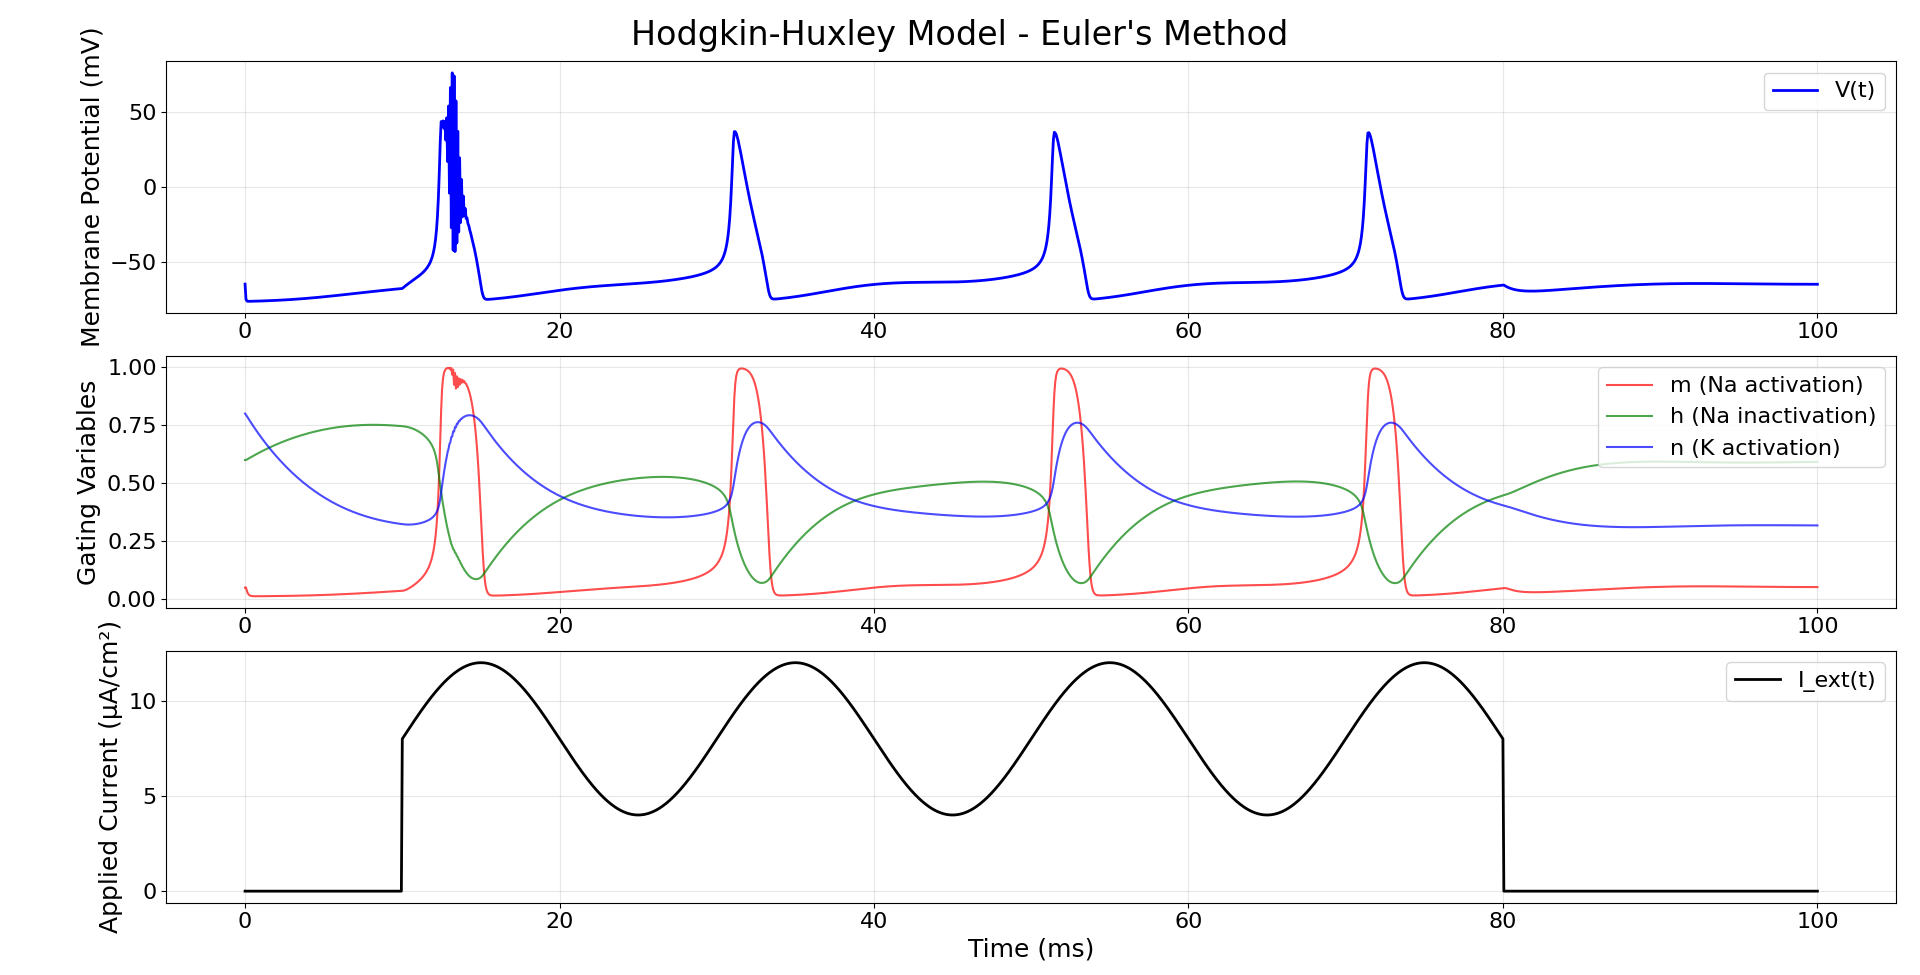
\includegraphics[width=0.8\linewidth]{Figs/euler-min-convergence.png}
        \caption{Solution instability as shown by the first spike using the Forward Euler method with a sinusoidal external current at its minimum convergence step ratio (17 steps/ms).}
        \label{fig:euler-min-convergence}
    \end{figure}

    \begin{multicols}{2}

\subsection{Signal Processing}
\label{subsec:signal-processing-results}

    To analyze the performance of the FIR filter, RMS error of the filtered signal was plotted against the noisy signal RMS error (Figure~\ref{fig:noise-rms-vs-filter-rms}).
    At low values of noise signal RMS the relationship appears stochastic. In this region, the RMS error of the filtered signal is dependent on input parameters from the various noise additives. 
    This behaviour is also dependent on the baseline error of the FIR filter, which is present even in the absence of noise. The baseline arises from quantization of input and coefficients from the software, and output truncation.
    As the noise RMS increases, namely with gaussian noise, the plot converges toward a linear relationship. The filter scales predictably with a slope of less than one, removing a constant fraction of noise power independent of noise amplitude. 


    \begin{minipage}{\linewidth}
        \centering
        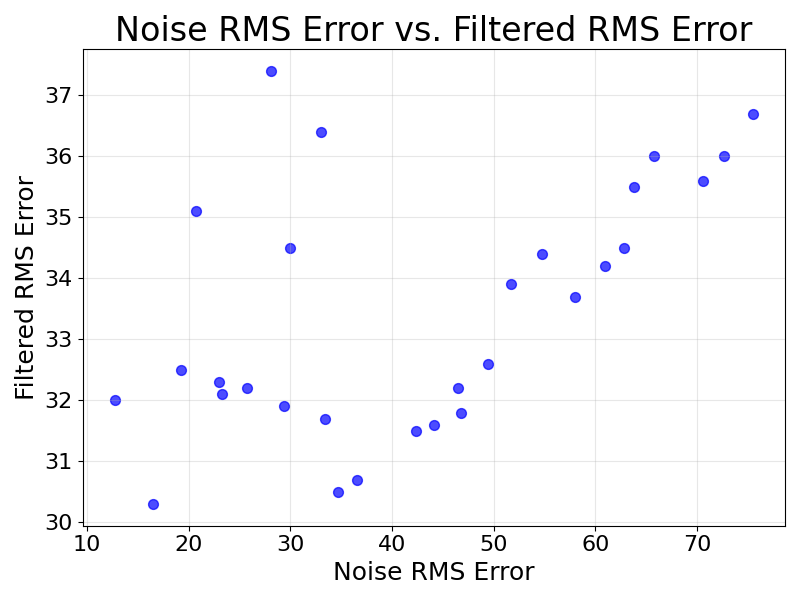
\includegraphics[width=0.8\linewidth]{Figs/noise-rms-vs-filter-rms.png}
        \captionof{figure}{RMS relationship, stochastic at low noise signal RMS but linearizes as signal gets noisier.}
        \label{fig:noise-rms-vs-filter-rms}
    \end{minipage}

    \end{multicols}

    \begin{figure}[ht]
        \centering
        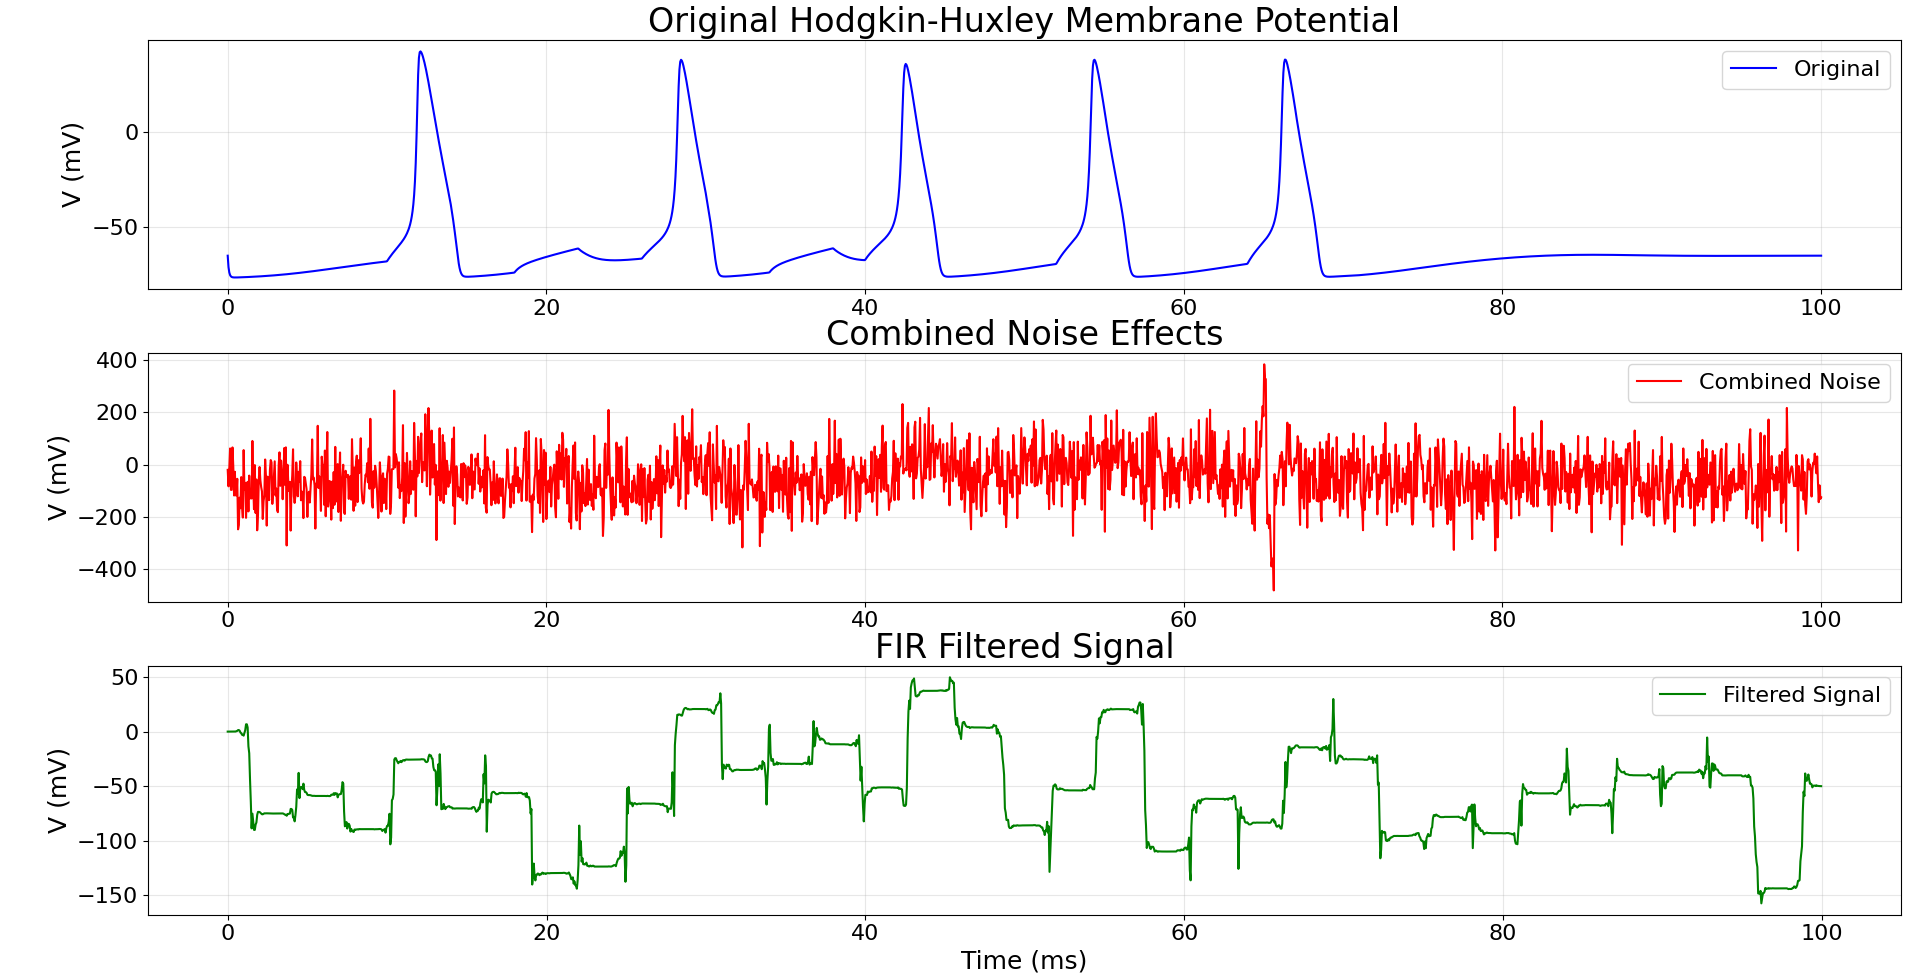
\includegraphics[width=0.8\linewidth]{Figs/fir-max-gaussian-std-filter.png}
        \caption{Insert caption about standard deviation of 90 in addition to amplitude modulation and ocular artifacts.}
        \label{fig:fir-max-guassian-std-filter}
    \end{figure}

    \begin{multicols}{2}

\subsection{Spike Detection}
\label{subsec:spike-detection-results}

    Even in the presence of significant noise, action potential spikes are reliably detected in the FIR-filtered signal and the spike times align with the peaks of the membrane potential. 
    The detection theshold ensures true spikes are captured while ignoring noise fluctuations.
    Temporal distribution of spikes within expectation of the model's firing patterns were observed.
    False positives cause shorter intervals and false negatives cause larger intervals, but overall were consistent with the original Hodgkin-Huxley membrane potential.
    
    \end{multicols}

    \begin{figure}[ht]
        \centering
        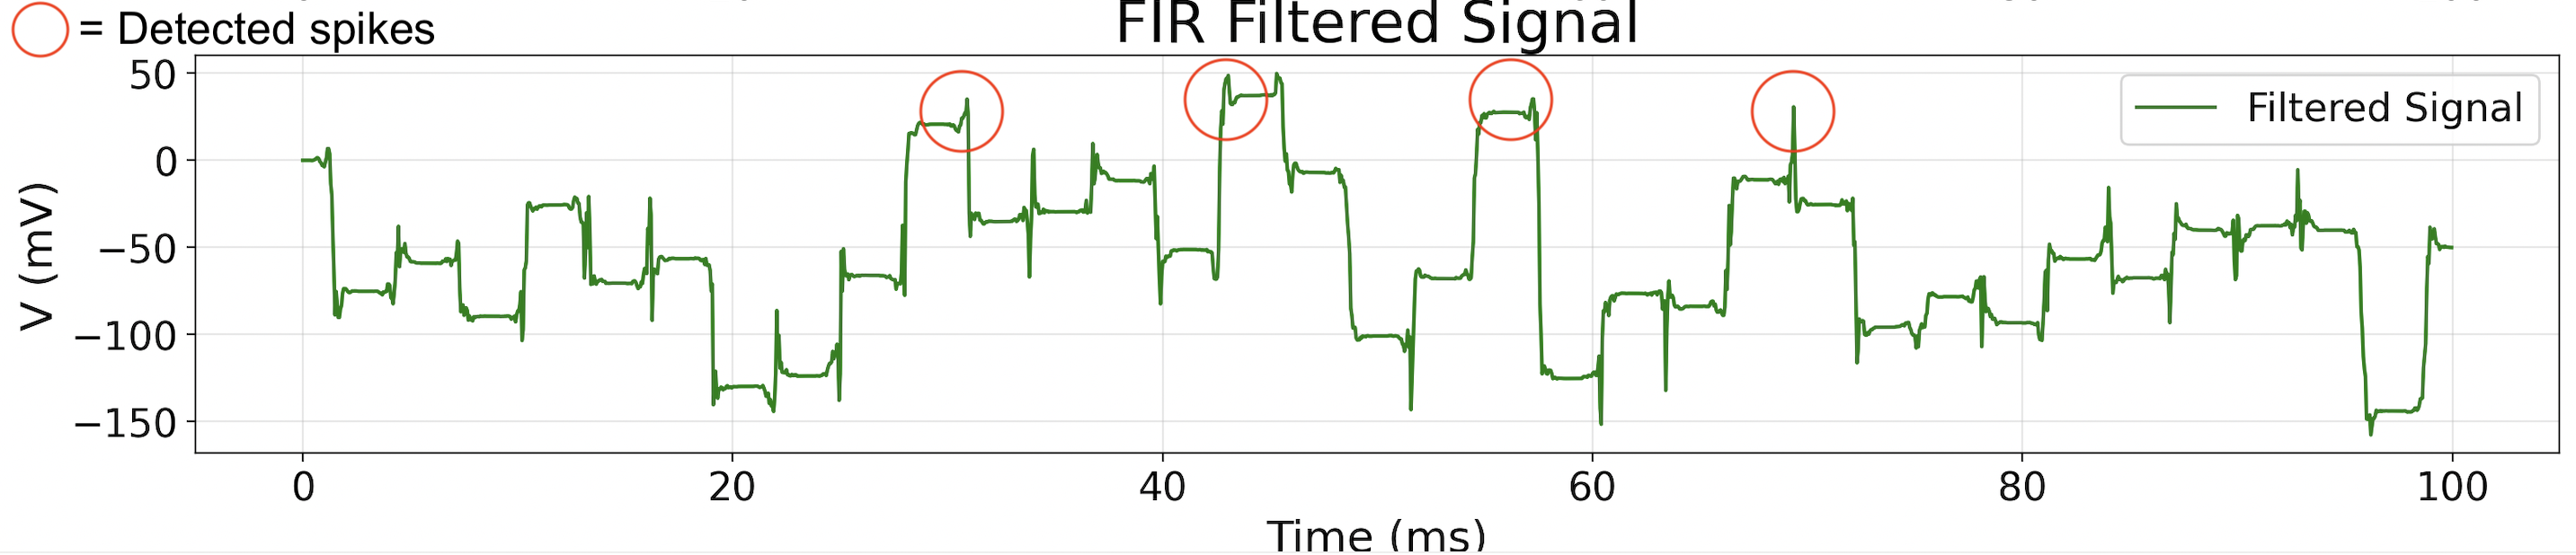
\includegraphics[width=0.8\linewidth]{Figs/FIR_detected_spikes.png}
        \caption{Detected spikes within the FIR filtered signal. Three spikes were correctly detected while one was an incorrectly detected false positive.}
        \label{fig:fir-detected-spikes}
    \end{figure}

    \begin{multicols}{2}    

    In Figure {\ref{fig:fir-detected-spikes}}, the filtered signal shows four detected spikes at 28.65 ms, 42.75 ms, 55.40 ms, and 69.35 ms. 
    Computing the inter-spike intervals using np.diff yields values of 14.10 ms, 12.65 ms, and 13.95 ms, showing a nearly periodic firing pattern.
    This consistency confirms that spike detection is internally coherent.

    The spike times were compared with the ground truth. 
    The detector produced 4 spikes, 3 of which matched ground truth. 
    One event at 69.35 ms did not match the ground truth spike located at 66.35 ms, meaning it would be considered a false positive (and the ground-truth spike a false negative).

    \end{multicols}